\section{System design choices}
\subsection{Overview}


The overall system needed to accomplish the following high-level tasks
\begin{itemize}
  \item Detect exceptions and extract values of variables on the stack-trace
  \item Store the captured data for later analysis
  \item Provide a useful visualisation of extracted data
\end{itemize}

With these primordial functions in mind, four main components evolved
\begin{enumerate}
  \item An Agent attached to every JVM instance which can capture the data
  \item An API to which the Agent send the data
  \item A Database with which the API engine can interact to store and read data
  \item and a Dashboard Portal that connects to the API and provides a view-port into the collected and processed data
\end{enumerate}

A micro-service pattern has been considered when designing this service suite \cite{microservices}. All of the components are built in different programming languages and can be deployed independently as long as the versions in production have common communication interfaces or are otherwise backward compatible with each other.

The agent itself is a micro-service towards the JVM it is observing. It runs as a separate process and it can be attached at any point in the lifetime of the JVM.

\begin{figure}[H]
  \centering
    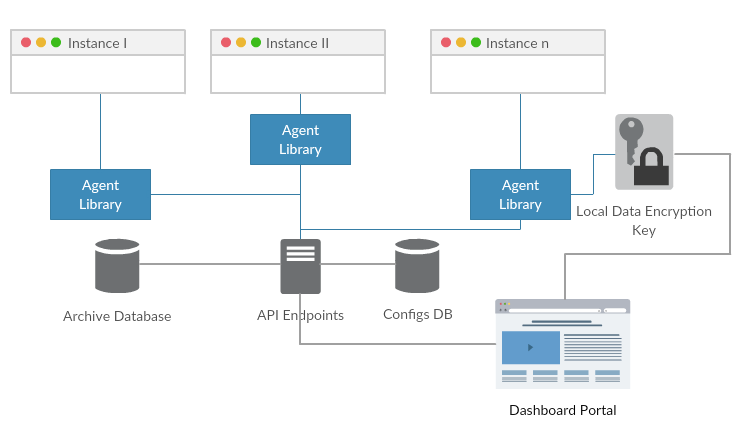
\includegraphics[width=\textwidth]{initial-design.png} 
  \caption[Initial system design diagram]{The initial system design, before the start of implementation.}

\end{figure} 

The initial system design included a configuration database which would allow the user to configure properties of how the agent behaved through the Dashboard Portal. Moreover, it factored in the way encryption may be accounted for. As we shall see in the next section, these parts have been excluded from the core for the purpose of finishing a base version before further improvements are considered.

\subsection{Revised and final system components} 

\begin{figure}[H]
  \centering
    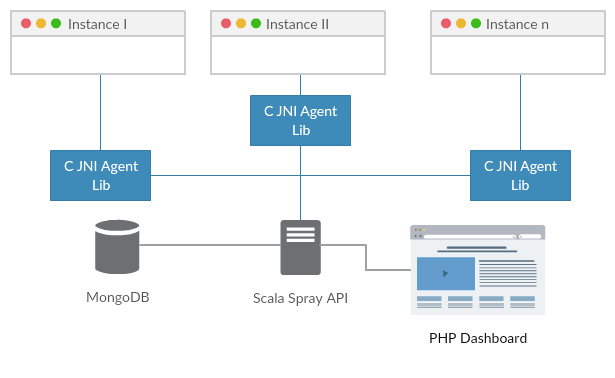
\includegraphics[width=\textwidth]{end-design.png} 
  \caption[Revised system design diagram]{The revised system design, as an artefact after the end of implementation.}

\end{figure}

After going through a few revisions in the lifetime of the project, the final system has been implemented following this design:



The reasons why each of the components has been developed in the mentioned programming language are explored in the next section.

\subsection{Agent Library}
\subsubsection{Overview}

This component is focused on using the JNI and JVMTI to obtain data from the JVM. More specifically, its purpose is to capture a relevant slice of the variable-tree and use the JVMTI exception callback to decide when to record this data. One of these cases being when an exception has been detected.

The agent must have access to explore the stack-trace and the ability to match variable data to the methods present on the stack trace.

\subsubsection{Technology choice}

\begin{figure}[H]
  \centering
    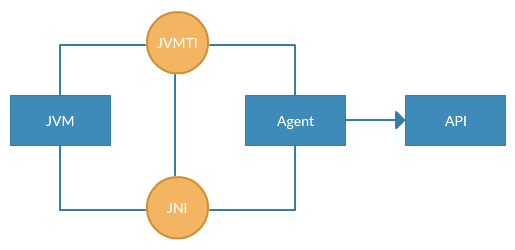
\includegraphics[width=\textwidth]{jvmti.png} 
  \caption[JVMTI and JNI provide access for the Native Agent to the JVM]{JVMTI and JNI provide access for the Native Agent into the JVM}

\end{figure} 

Two main options were considered: a Java agent versus a Native agent.

A Java agent cannot access low-level aspects of the JVM with as much ease as a native one and it cannot run as a separate process which means that if it crashes it crashes the JVM as well. Moreover, because the Java agent becomes part of the JVM, it has impact on the garbage collection and JVM performance, possibly impacting its behaviour in unwanted ways and altering results of other tools the user may be using to analyse resource usage of the app \cite{javavsnativetaki,javavsnativetdyna}.

There are many libraries already built for Java based agents, such as Javaassist \cite{javassist} and ASM \cite{asm}, but their main goals is dynamic bytecode manipulation and given the aims of the project, a native mainly read-only agent made more sense.

A native agent would also be loaded before the JVM loads any classes and stopped after the JVM has wrapped everything up, while the Java based agent is loaded at a later stage in the lifetime of the JVM \cite{javavsnativetdyna}.

The Instrumentation package to which a Java agent would have access to is only for the instrumentation functionality of the JVMTI \cite{jvmtiInterface}.

A native agent has unrestricted access to the lowest level of instrumentation and can most efficiently dig deep into the depths of the JVM. By doing its own memory allocations in the shared memory outside of the managed heap, it allows for a small overhead and no impact into JVM garbage collection time.

The native access has direct native access to the JNI and JVMTI.

\subsubsection{Conclusion}
A native agent implementation using the JNI and JVMTI interfaces is the choice that best matches the scope of this project. 

\subsection{Database}
\subsubsection{Overview}
The database engine needs to be able to handle concurrent writes but not particularly to the same object as once the data for a stack-trace is recorded, it is never updated.

Advanced filtering is also not very important. Simple queries would be enough to serve the purposes of the current system, such as filtering by the originating app.

At this prototype level, a preference to a flexible structure for stored entries is preferred.

\subsubsection{Technology choice}
There were many approaches which could be taken for the log storage engine. Specialised tools for storing log-like data could have been used, such as Logstash \cite{logstash}, which would provide good interfaces for analysing the data and handling concurrent writes.

Graph-based database engines were also a consideration and might provide specific advantages for future versions of this product, when its ability to scale into handling multiple instances of apps improves.

However, more traditional engines were considered as the main choices in order to easily provide storage for the user, configuration and session data through the same engine.

While servers such as MySQL and MSSQL would have offered better querying capabilities and would be the better choices when storing entities which relate to one another to avoid duplication, NoSQL-like engines matched the project's iterative changing requirements better.

MongoDB is a well documented and flexible engine with adaptors built in most popular programming languages including the choices made for this project. 

\subsubsection{Conclusion}
MongoDB was picked based of familiarity, documentation and flexibility.

\subsection{API}
\subsubsection{Overview}
An Application Programming Interface, referred to as the API, will be provided, sitting at the centre of the system. The Agents communicate with this service to store data and the Dashboard accesses the service on order to obtain it.

Authentication for the dashboard will be done via a token-based session management approach and the agents will use an API key and App key to relate the specific data they register to a specific user configured app.

Currently, multiple instances of the same app would use the same App key.

\subsubsection{Technology choice}
A RESTful HTTP API design \cite{rest} has been used as the particular kind of usage we are in scope of did not need a continuous connection or server to client communication such as say Sockets could accommodate. Moreover, the API and App keys provide a sufficiently secure level of authentication for each request.

But Sockets could be an interesting choice in the future for agents to locally communicate with one another, especially agents attached to different instances of the same app, which could avoid recording the same stack-traces by locally exchanging information.

There are numerous frameworks for most programming languages which can serve as an API base. As such, it is very hard to attempt to select the very best choice and the selection process ended up considering aspects such as developer familiarity with the programming language.

NodeJS and Python were the initial candidates. However, they were both outranked by Scala for the same reason, which is the lack of a default typed environment (strict definitions for variables and compile-time detection of potential type-related mistakes) \cite{scalaVSjsRH}. The advantage of a typed language out-weighted the shorter development time.

NodeJS, for example, has Typescript as a way to work-around this problem.

Scala has been steadily gaining terrain in the enterprise world and is trusted by developers. Given also that the kind of data meant to be recorded (log-like) is often never altered it is ideal for a functional programming language.

One other interesting part about having a JVM (Scala) based component would be the ability to run the end product (the agent) on it. However, the project has not reached this phase at this time.

\subsubsection{Conclusion}
The Scala Spray framework combined with SBT for dependency management ended up being the technology choice for this component.

\subsection{Dashboard Portal}
\subsubsection{Overview}
The purpose of this component is to allow the user actor to view data extracted by the agent in an intractable and friendly manner.

The dashboard talks to the API to create user sessions and obtain data. It would likely have to do some processing of the data itself in order to extract further information and the frontend might have to be encryption-aware in order to use local decryption keys to render protected data.

\subsubsection{Technology choice}

For this prototype and considering how little work the dashboard had to do, the decision to use PHP as the backend was made.


\subsubsection{Conclusion}
A Model-View-Controller framework named FuelPHP was used for separation of concerns and the in-built HTTP request framework handled the communication with the API.

The Twitter Bootstrap framework was used as a start for the design and multiple libraries can provide additional functionality such as encryption and decryption.

\newpage